%
% char.tex -- Charakteristiken einer hyperbolischen DGL
%
% (c) 2018 Prof Dr Andreas Müller, Hochschule Rapperswi
%
\documentclass[tikz]{standalone}
\usepackage{amsmath}
\usepackage{times}
\usepackage{txfonts}
\usepackage[utf8]{inputenc}
\usepackage{graphics}
\usepackage{ifthen}
\usepackage{color}
\usetikzlibrary{arrows,intersections}
\begin{document}
\definecolor{darkgreen}{rgb}{0,0.6,0}

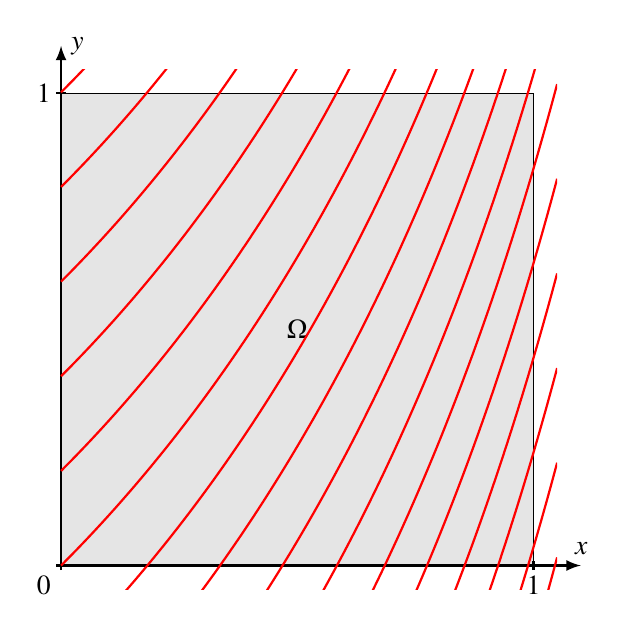
\begin{tikzpicture}[>=latex,thick,scale=6]
\fill[color=gray!20] (0,0) rectangle (1,1);
\draw[line width=0.1pt] (0,0)--(1,0)--(1,1)--(0,1)--cycle;
\draw[->] (-0.01,0) -- (1.1,0) coordinate[label={$x$}];
\draw[->] (0,-0.01) -- (0,1.1) coordinate[label={right:$y$}];
\node at (0.5,0.5) {$\Omega$};
\node at (0,0) [below left] {$0$};
\draw (1,-0.01)--(1,0.01);
\node at (1,0) [below] {$1$};
\draw (-0.01,1)--(0.01,1);
\node at (0,1) [left] {$1$};
\begin{scope}
\clip (-0.05,-0.05) rectangle (1.05,1.05);
\foreach \yoffset in {-3,-2.8,...,1}{
	\begin{scope}[yshift={\yoffset*28.5}]
		\draw[color=red] (0,0)
--(0.0105,0.0106)
--(0.0210,0.0212)
--(0.0315,0.0320)
--(0.0420,0.0429)
--(0.0525,0.0539)
--(0.0630,0.0650)
--(0.0735,0.0763)
--(0.0840,0.0876)
--(0.0945,0.0991)
--(0.1050,0.1107)
--(0.1155,0.1224)
--(0.1260,0.1343)
--(0.1365,0.1463)
--(0.1470,0.1584)
--(0.1575,0.1706)
--(0.1680,0.1830)
--(0.1785,0.1955)
--(0.1890,0.2081)
--(0.1995,0.2209)
--(0.2100,0.2338)
--(0.2205,0.2468)
--(0.2310,0.2600)
--(0.2415,0.2733)
--(0.2520,0.2868)
--(0.2625,0.3004)
--(0.2730,0.3142)
--(0.2835,0.3281)
--(0.2940,0.3422)
--(0.3045,0.3564)
--(0.3150,0.3708)
--(0.3255,0.3853)
--(0.3360,0.4001)
--(0.3465,0.4149)
--(0.3570,0.4300)
--(0.3675,0.4452)
--(0.3780,0.4605)
--(0.3885,0.4761)
--(0.3990,0.4918)
--(0.4095,0.5077)
--(0.4200,0.5238)
--(0.4305,0.5401)
--(0.4410,0.5566)
--(0.4515,0.5733)
--(0.4620,0.5901)
--(0.4725,0.6072)
--(0.4830,0.6244)
--(0.4935,0.6419)
--(0.5040,0.6596)
--(0.5145,0.6775)
--(0.5250,0.6956)
--(0.5355,0.7139)
--(0.5460,0.7325)
--(0.5565,0.7512)
--(0.5670,0.7703)
--(0.5775,0.7895)
--(0.5880,0.8090)
--(0.5985,0.8287)
--(0.6090,0.8487)
--(0.6195,0.8690)
--(0.6300,0.8895)
--(0.6405,0.9103)
--(0.6510,0.9314)
--(0.6615,0.9527)
--(0.6720,0.9743)
--(0.6825,0.9962)
--(0.6930,1.0185)
--(0.7035,1.0410)
--(0.7140,1.0638)
--(0.7245,1.0870)
--(0.7350,1.1104)
--(0.7455,1.1343)
--(0.7560,1.1584)
--(0.7665,1.1829)
--(0.7770,1.2078)
--(0.7875,1.2330)
--(0.7980,1.2586)
--(0.8085,1.2846)
--(0.8190,1.3111)
--(0.8295,1.3379)
--(0.8400,1.3651)
--(0.8505,1.3928)
--(0.8610,1.4209)
--(0.8715,1.4494)
--(0.8820,1.4785)
--(0.8925,1.5080)
--(0.9030,1.5380)
--(0.9135,1.5685)
--(0.9240,1.5996)
--(0.9345,1.6312)
--(0.9450,1.6634)
--(0.9555,1.6961)
--(0.9660,1.7294)
--(0.9765,1.7634)
--(0.9870,1.7980)
--(0.9975,1.8333)
--(1.0080,1.8693)
--(1.0185,1.9060)
--(1.0290,1.9434)
--(1.0395,1.9816)
--(1.0500,2.0206)
;

		\def\gruen{\draw[color=darkgreen] (0,0)
--(0.0100,-0.0041)
--(0.0200,-0.0083)
--(0.0300,-0.0125)
--(0.0400,-0.0167)
--(0.0500,-0.0209)
--(0.0600,-0.0251)
--(0.0700,-0.0294)
--(0.0800,-0.0336)
--(0.0900,-0.0379)
--(0.1000,-0.0422)
--(0.1100,-0.0465)
--(0.1200,-0.0508)
--(0.1300,-0.0551)
--(0.1400,-0.0595)
--(0.1500,-0.0638)
--(0.1600,-0.0682)
--(0.1700,-0.0726)
--(0.1800,-0.0770)
--(0.1900,-0.0815)
--(0.2000,-0.0859)
--(0.2100,-0.0904)
--(0.2200,-0.0949)
--(0.2300,-0.0994)
--(0.2400,-0.1039)
--(0.2500,-0.1084)
--(0.2600,-0.1129)
--(0.2700,-0.1175)
--(0.2800,-0.1221)
--(0.2900,-0.1267)
--(0.3000,-0.1313)
--(0.3100,-0.1360)
--(0.3200,-0.1406)
--(0.3300,-0.1453)
--(0.3400,-0.1500)
--(0.3500,-0.1547)
--(0.3600,-0.1594)
--(0.3700,-0.1642)
--(0.3800,-0.1690)
--(0.3900,-0.1737)
--(0.4000,-0.1785)
--(0.4100,-0.1834)
--(0.4200,-0.1882)
--(0.4300,-0.1931)
--(0.4400,-0.1980)
--(0.4500,-0.2029)
--(0.4600,-0.2078)
--(0.4700,-0.2128)
--(0.4800,-0.2177)
--(0.4900,-0.2227)
--(0.5000,-0.2277)
--(0.5100,-0.2327)
--(0.5200,-0.2378)
--(0.5300,-0.2429)
--(0.5400,-0.2480)
--(0.5500,-0.2531)
--(0.5600,-0.2582)
--(0.5700,-0.2634)
--(0.5800,-0.2686)
--(0.5900,-0.2738)
--(0.6000,-0.2790)
--(0.6100,-0.2842)
--(0.6200,-0.2895)
--(0.6300,-0.2948)
--(0.6400,-0.3001)
--(0.6500,-0.3055)
--(0.6600,-0.3108)
--(0.6700,-0.3162)
--(0.6800,-0.3216)
--(0.6900,-0.3271)
--(0.7000,-0.3325)
--(0.7100,-0.3380)
--(0.7200,-0.3435)
--(0.7300,-0.3491)
--(0.7400,-0.3546)
--(0.7500,-0.3602)
--(0.7600,-0.3658)
--(0.7700,-0.3715)
--(0.7800,-0.3771)
--(0.7900,-0.3828)
--(0.8000,-0.3885)
--(0.8100,-0.3943)
--(0.8200,-0.4001)
--(0.8300,-0.4059)
--(0.8400,-0.4117)
--(0.8500,-0.4175)
--(0.8600,-0.4234)
--(0.8700,-0.4293)
--(0.8800,-0.4353)
--(0.8900,-0.4412)
--(0.9000,-0.4472)
--(0.9100,-0.4533)
--(0.9200,-0.4593)
--(0.9300,-0.4654)
--(0.9400,-0.4715)
--(0.9500,-0.4777)
--(0.9600,-0.4839)
--(0.9700,-0.4901)
--(0.9800,-0.4963)
--(0.9900,-0.5026)
--(1.0000,-0.5089)
--(1.0100,-0.5152)
--(1.0200,-0.5216)
--(1.0300,-0.5280)
--(1.0400,-0.5344)
--(1.0500,-0.5409)
;}
\def\gruenundef{\fill[color=darkgreen!20] (0,1)
--(0.0100,0.9959)
--(0.0200,0.9917)
--(0.0300,0.9875)
--(0.0400,0.9833)
--(0.0500,0.9791)
--(0.0600,0.9749)
--(0.0700,0.9706)
--(0.0800,0.9664)
--(0.0900,0.9621)
--(0.1000,0.9578)
--(0.1100,0.9535)
--(0.1200,0.9492)
--(0.1300,0.9449)
--(0.1400,0.9405)
--(0.1500,0.9362)
--(0.1600,0.9318)
--(0.1700,0.9274)
--(0.1800,0.9230)
--(0.1900,0.9185)
--(0.2000,0.9141)
--(0.2100,0.9096)
--(0.2200,0.9051)
--(0.2300,0.9006)
--(0.2400,0.8961)
--(0.2500,0.8916)
--(0.2600,0.8871)
--(0.2700,0.8825)
--(0.2800,0.8779)
--(0.2900,0.8733)
--(0.3000,0.8687)
--(0.3100,0.8640)
--(0.3200,0.8594)
--(0.3300,0.8547)
--(0.3400,0.8500)
--(0.3500,0.8453)
--(0.3600,0.8406)
--(0.3700,0.8358)
--(0.3800,0.8310)
--(0.3900,0.8263)
--(0.4000,0.8215)
--(0.4100,0.8166)
--(0.4200,0.8118)
--(0.4300,0.8069)
--(0.4400,0.8020)
--(0.4500,0.7971)
--(0.4600,0.7922)
--(0.4700,0.7872)
--(0.4800,0.7823)
--(0.4900,0.7773)
--(0.5000,0.7723)
--(0.5100,0.7673)
--(0.5200,0.7622)
--(0.5300,0.7571)
--(0.5400,0.7520)
--(0.5500,0.7469)
--(0.5600,0.7418)
--(0.5700,0.7366)
--(0.5800,0.7314)
--(0.5900,0.7262)
--(0.6000,0.7210)
--(0.6100,0.7158)
--(0.6200,0.7105)
--(0.6300,0.7052)
--(0.6400,0.6999)
--(0.6500,0.6945)
--(0.6600,0.6892)
--(0.6700,0.6838)
--(0.6800,0.6784)
--(0.6900,0.6729)
--(0.7000,0.6675)
--(0.7100,0.6620)
--(0.7200,0.6565)
--(0.7300,0.6509)
--(0.7400,0.6454)
--(0.7500,0.6398)
--(0.7600,0.6342)
--(0.7700,0.6285)
--(0.7800,0.6229)
--(0.7900,0.6172)
--(0.8000,0.6115)
--(0.8100,0.6057)
--(0.8200,0.5999)
--(0.8300,0.5941)
--(0.8400,0.5883)
--(0.8500,0.5825)
--(0.8600,0.5766)
--(0.8700,0.5707)
--(0.8800,0.5647)
--(0.8900,0.5588)
--(0.9000,0.5528)
--(0.9100,0.5467)
--(0.9200,0.5407)
--(0.9300,0.5346)
--(0.9400,0.5285)
--(0.9500,0.5223)
--(0.9600,0.5161)
--(0.9700,0.5099)
--(0.9800,0.5037)
--(0.9900,0.4974)
--(1.0000,0.4911)
--(1,1)--cycle;
}

	\end{scope}
}
\end{scope}
\end{tikzpicture}

\end{document}
